\documentclass{article}

\usepackage{graphicx}
\usepackage{tikz}
\usepackage{tikzsymbols}
\usetikzlibrary{calc,patterns,shapes.geometric}
\pagestyle{empty}
\usepackage[margin=0pt]{geometry}
\geometry{papersize={14in,12in}}

\def\centerarc[#1](#2)(#3:#4:#5){\draw[#1] ($(#2)+({#5*cos(#3)},{#5*sin(#3)})$) arc (#3:#4:#5);}

\begin{document}
	\begin{figure}
		\centering
		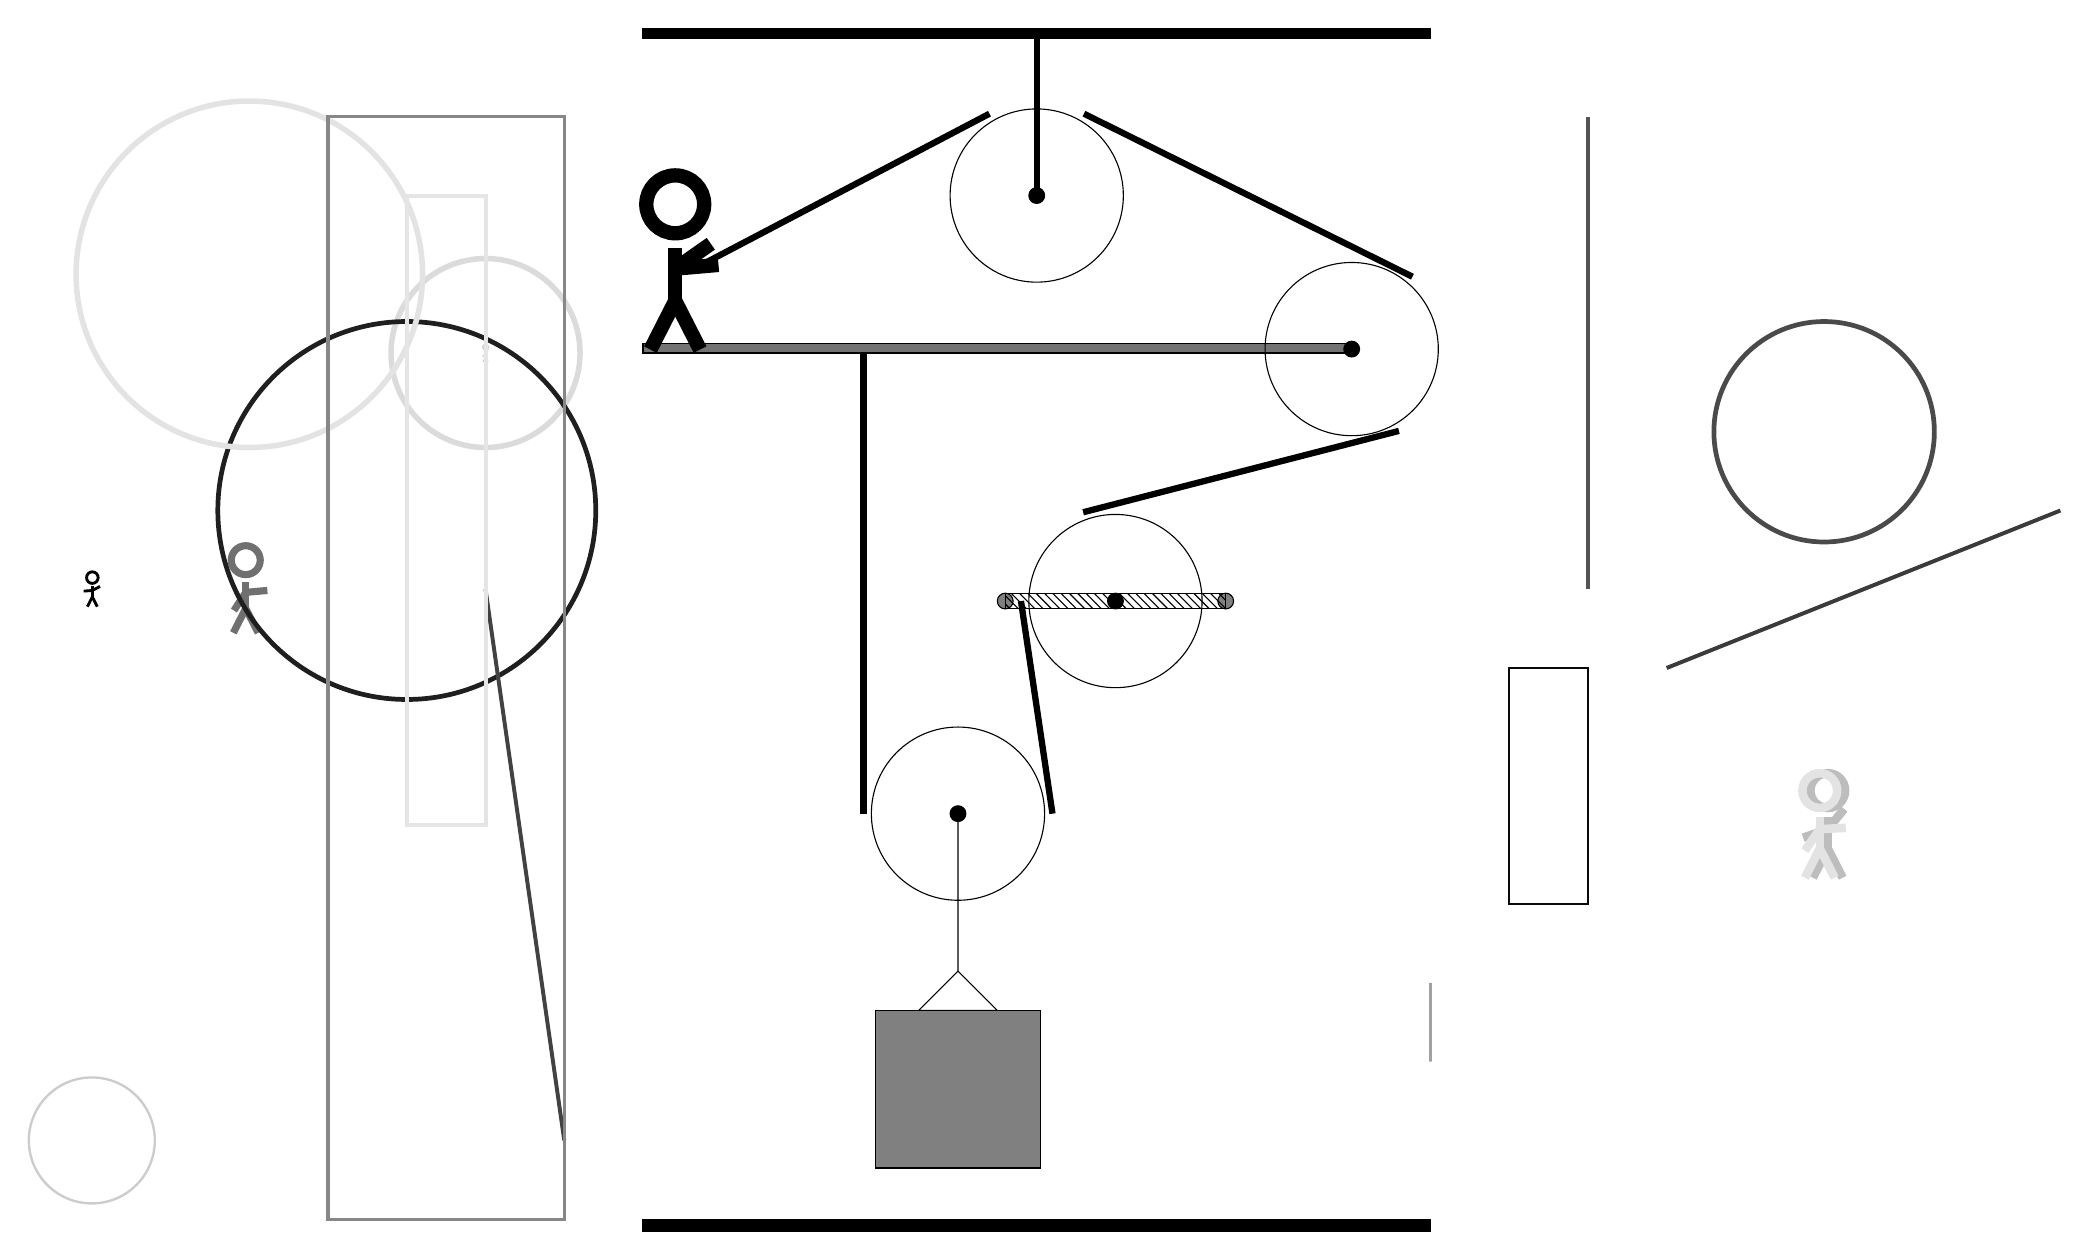
\begin{tikzpicture}
			%%%%% START %%%%%
			
			\draw[fill=black] (-2, 13) rectangle (8, 13.125);
			
			\draw[fill=black!55] (-2, 9) rectangle (7, 9.125);
			
			\draw (2, 3.15) circle (1.1);
			\draw[fill=black] (2, 3.15) circle (0.1);
			
			\draw (7, 9.05) circle (1.1);
			\draw[fill=black] (7, 9.05) circle (0.1);
			
			\draw[fill=white](4, 5.85) circle (1.1);
			\draw[fill=black] (4, 5.85) circle (0.1);
			\draw[fill=black!50] (2.6, 5.85) circle (0.1);
			\draw[fill=black!50] (5.4, 5.85) circle (0.1);
			\draw[pattern=north west lines, pattern color=black] (2.6, 5.95) rectangle (5.4, 5.75);
			
			\draw (3, 11) circle (1.1);
			\draw[fill=black] (3, 11) circle (0.1);
			\draw[line width=0.8mm] (3, 11) -- (3, 13);
			
			\draw (2, 3.15) -- (2, 1.15) -- (1.5, 0.65) -- (2.5, 0.65) -- (2, 1.15);
			\draw[fill=black!50] (0.95, 0.65) rectangle (3.05, -1.35);
			
			\draw[line width=0.2mm, color=black!96] (9, 2) rectangle (10, 5);
			
			\node[line width=0.6mm, color=black!26] at (13, 3) {\Strichmaxerl[6][19][51]};
			\draw [line width=0.7mm, color=black!14](-4, 9) circle (1.2);
			\node[line width=0.7mm, color=black!56] at (-7, 6) {\Strichmaxerl[5][57][5]};
			\draw[line width=0.4mm, color=black!37] (8, 0) rectangle (8, 1);
			\draw [line width=0.6mm, color=black!71](13, 8) circle (1.4);
			\draw[line width=0.5mm, color=black!77](11, 5) -- (16, 7);
			
			\draw [line width=0.5mm, color=black!93](-7, 2) circle (0.0);
			\draw [line width=0.6mm, color=black!88](-5, 7) circle (2.4);
			\node[line width=0.7mm, color=black!100] at (-9, 6) {\Strichmaxerl[2][4][28]};
			\draw[line width=0.5mm, color=black!74](-3, -1) -- (-4, 6);
			
			\draw [line width=0.7mm, color=black!11](-7, 10) circle (2.2);
			\draw[line width=0.4mm, color=black!47] (-3, 12) rectangle (-6, -2);
			
			\node[line width=0.7mm, color=black!18] at (-4, 9) {\Strichmaxerl[1][47][83]};
			\draw[line width=0.5mm, color=black!10] (-4, 3) rectangle (-5, 11);
			\node[line width=0.6mm, color=black!11] at (13, 3) {\Strichmaxerl[6][55][3]};
			
			\draw[line width=0.5mm, color=black!67](10, 6) -- (10, 12);
			\draw [line width=0.3mm, color=black!20](-9, -1) circle (0.8);
			
			\draw[line width=0.8mm] (0.8, 9) -- (0.8, 3.15);
			\centerarc[line width=0.8mm](2, 3.15)(180:360:1.2000000000000002);
			\draw[line width=0.8mm](3.2, 3.15) -- (2.8, 5.85);
			\centerarc[line width=0.8mm](4, 5.85)(110:180:1.2000000000000002);
			\draw[line width=0.8mm](3.5896, 6.9776) -- (7.6, 8.0108);
			\centerarc[line width=0.8mm](7, 9.05)(-60:50:1.2000000000000002);
			\draw[line width=0.8mm](7.7714, 9.9692) -- (3.6, 12.0392);
			\centerarc[line width=0.8mm](3, 11)(60:120:1.2000000000000002);
			\draw[line width=0.8mm](2.4, 12.0392) -- (-1.2, 10.15);
			
			\node at (-1.5, 10.15) {\Strichmaxerl[10][-175][35]};
			
			\draw[fill=black] (-2, -2) rectangle (8, -2.15);
			
			%%%%% END %%%%%
		\end{tikzpicture}
	\end{figure}	
\end{document}